
\documentclass[12pt]{article}

% Layout.
\usepackage[top=1in, bottom=0.75in, left=1in, right=1in, headheight=1in, headsep=6pt]{geometry}

% Fonts.
\usepackage{mathptmx}
\usepackage[scaled=0.86]{helvet}
\renewcommand{\emph}[1]{\textsf{\textbf{#1}}}

% TiKZ.
\usepackage{tikz, pgfplots}
\usetikzlibrary{calc}
\pgfplotsset{compat = newest}
 
\pgfplotsset{my style/.append style={axis x line=middle, axis y line=
middle, xlabel={$x$}, ylabel={$y$}, axis equal }}

% Misc packages.
\usepackage{amsmath,amssymb,latexsym}
\usepackage{graphicx}
\usepackage{array}
\usepackage{xcolor}
\usepackage{multicol}

% Commands to set various header/footer components.
\makeatletter
\def\doctitle#1{\gdef\@doctitle{#1}}
\doctitle{Use {\tt\textbackslash doctitle\{MY LABEL\}}.}
\def\docdate#1{\gdef\@docdate{#1}}
\docdate{Use {\tt\textbackslash docdate\{MY DATE\}}.}
\def\doccourse#1{\gdef\@doccourse{#1}}
\let\@doccourse\@empty
\def\docscoring#1{\gdef\@docscoring{#1}}
\let\@docscoring\@empty
\def\docversion#1{\gdef\@docversion{#1}}
\let\@docversion\@empty
\makeatother

% Headers and footers layout.
\makeatletter
\usepackage{fancyhdr}
\pagestyle{fancy}
\fancyhf{} % Clears all headers/footers.
\lhead{\baselineskip 30pt
%\emph{\@doctitle\hfill\@docdate}
\emph{\@docdate\hfill\@doctitle}
\ifnum \value{page} > 1\relax\else\\
\emph{Name: \rule{3.5in}{1pt}\hfill \@docscoring}\fi}
\rfoot{\emph{\@docversion}}
\lfoot{\emph{\@doccourse}}
\cfoot{\emph{\thepage}}
\renewcommand{\headrulewidth}{0pt}%
\makeatother

% Paragraph spacing
\parindent 0pt
\parskip 6pt plus 1pt

% A problem is a section-like command. Use \problem{5} to
% start a problem worth 5 points.
\newcounter{probcount}
\newcounter{subprobcount}
\setcounter{probcount}{0}
\newcommand{\problem}[1]{%
\par
\addvspace{4pt}%
\setcounter{subprobcount}{0}%
\stepcounter{probcount}%
\makebox[0pt][r]{\emph{\arabic{probcount}.}\hskip1ex}\emph{[#1 points]}\hskip1ex}
\newcommand{\thesubproblem}{\emph{\alph{subprobcount}.}}

% Subproblems are an enumerate-like environment with a consistent
% numbering scheme. 
% Use \begin{subproblems}\item...\item...\end{subproblems}
\newenvironment{subproblems}{%
\begin{enumerate}%
\setcounter{enumi}{\value{subprobcount}}%
\renewcommand{\theenumi}{\emph{\alph{enumi}}}}%
{\setcounter{subprobcount}{\value{enumi}}\end{enumerate}}

% Blanks for answers in normal and math mode.
\newcommand{\blank}[1]{\rule{#1}{0.75pt}}
\newcommand{\mblank}[1]{\underline{\hspace{#1}}}
\def\emptybox(#1,#2){\framebox{\parbox[c][#2]{#1}{\rule{0pt}{0pt}}}}

% Misc.
\renewcommand{\d}{\displaystyle}
\newcommand{\ds}{\displaystyle}
\def\bc{\begin{center}}
\def\ec{\end{center}}
\def\be{\begin{enumerate}}
\def\ee{\end{enumerate}}


\doctitle{Math 251: Quiz 5}
\docdate{October 7, 2021}
\doccourse{UAF Calculus I}
\docversion{v-1}
\docscoring{\blank{0.8in} / 25}
\begin{document}

There are 25 points possible on this quiz. No aids (book, calculator, etc.)
are permitted.  {\emph{Show all work for full credit.}}

\problem{16} Find $\displaystyle{\large{\frac{dy}{dx}}}.$ You do not have to simplify
	\begin{subproblems}
	\item $y=\cos^{-1}(\sqrt{x})$ %(\S 3.7 \# 279)
	\vfill
	\item $y=\left( x+ \sin^{-1}(x) \right)^5$ %(\S 3.7 \# 283)
	\vfill
	\item $y=e^{2x}\cos(x)$ %(\S 3.9 \#331,331,333)
	\vfill
	\item $y=\ln(8x+1)$ %(\S 3.9 \# 340, 341)
	\vfill
	\end{subproblems}
\newpage
\problem{5} The graph of $x^4y-xy^3=2$ is sketched below. %(\S 3.8 \# 313, 317)\\

\begin{multicols}{2}

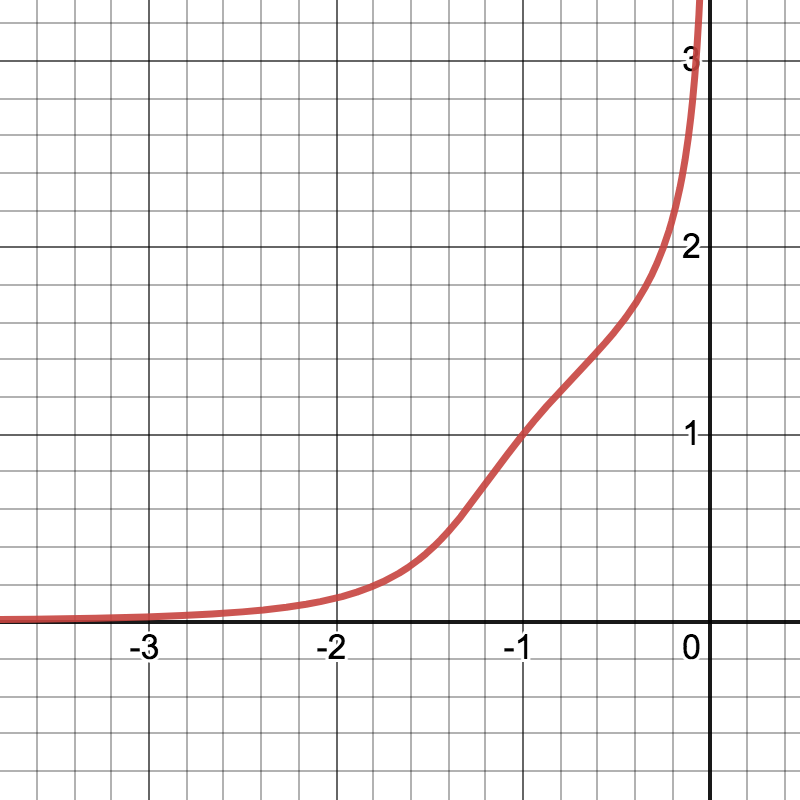
\includegraphics[scale=0.2]{M251F21_Q6_pic.png}
	
	(a) Find $dy/dx.$
\end{multicols} 

(b) Write an equation for the line \emph{normal} to the curve at the point $(-1,1)$ and \emph{sketch} the line on the graph.

	\vfill
	
	
\problem{4} Find the derivative of $y=(x)^{\sin(x)}.$ (Recall that you will have to use \emph{logarithmic differentiation}.) %\S 3.9 \# 347,348 and \S 3.8)
\vspace{2.5in}
\end{document}